\part{Week 7}
\chapter{The quantum Fourier transform and its applications}
We'll study \textit{quantum Fourier transform}, which is a class of problems quantum computers are more efficient in than classical computers.

\section{The quantum Fourier transform}
The \textit{discrete Fourier transform} takes a vector of complex numbers $x_0,\dots,x_{N-1}$ of complex numbers and outputs a same length vector of complex numbers $y_0\dots,y_{N-1}$ given by
\begin{equation}
    y_k \equiv \frac{1}{\sqrt{N}}\sum_{j=0}^{N-1}x_je^{2\pi ijk/N}.
\end{equation}
The \textit{quantum Fourier transform} is exactly the same thing but with a different convention. The quantum Fourier transform on an orthonormal basis $\qo,\dots,\ket{N-1}$ is a linear operator which does
\begin{equation}
    \ket{j} \longrightarrow \frac{1}{\sqrt{N}}\sum_{j=0}^{N-1}\ket{k}e^{2\pi ijk/N}.
\end{equation}
which corresponds to
\begin{equation}
    \sum_{j=0}^{N-1}x_j\ket{j} \longrightarrow \sum_{k=0}^{N-1}y_k\ket{k}
\end{equation}
where $y_k$ are discrete fourier transforms of $x_j$. It's not obvious but this is a unitary transform, and thus can be implemented by a quantum computer efficiently.

If $N=2^n$ and we can write $\ket{j}$ in it's binary representation as $\ket{j_1,j_2,\dots, j_n}$ and we also write $0.j_lj_{l+1}\dots j_m$ as the \textit{binary fraction} $j_l/2+j_{l+1}/4 + \dots + j_m/2^{m-l+1}$ then the quantum Fourier transform in it's \textit{product notation} is
\begin{equation}
    \ket{j_1,\dots,j_n} \longrightarrow \frac{\left(\qo + e^{2\pi i 0.j_n}\qi \right)\left(\qo + e^{2\pi i 0.j_{n-1}j_n\qi}\right)\dots\left(\qo + e^{2\pi i 0.j_1j_2\cdots j_n}\qi\right)}{2^{n/2}}.
\end{equation}

The evidence of the above product representation is as followed:
\begin{align}
   \ket{j} &\rightarrow \frac{1}{2^{n/2}} \sum_{k=0}^{2^n-1} e^{2\pi i j k / 2^n} \ket{k} \\
    &= \frac{1}{2^{n/2}} \sum_{k_1=0}^1 \dots \sum_{k_n=0}^1 e^{2\pi i j (\sum_{l=1}^n k_l2^{-l}) / 2^n} \ket{k_1 \dots k_n} \\
    &= \frac{1}{2^{n/2}} \sum_{k_1=0}^1 \dots \sum_{k_n=0}^1 \bigotimes_{l=1}^n e^{2\pi i j k_l 2^{-l}} \ket{k_l} \\
    &= \frac{1}{2^{n/2}} \bigotimes_{l=1}^n \left[ \sum_{k_l=0}^1 e^{2\pi i j k_l 2^{-l}} \ket{k_l} \right]\\
    &= \frac{1}{2^{n/2}} \bigotimes_{l=1}^n \left[ \ket{0} + e^{2\pi i j 2^{-l}} \ket{1} \right] \\
    &= \frac{\left(\qo + e^{2\pi i 0.j_n}\qi \right)\left(\qo + e^{2\pi i 0.j_{n-1}j_n\qi}\right)\dots\left(\qo + e^{2\pi i 0.j_1j_2\cdots j_n}\qi\right)}{2^{n/2}}. 
\end{align}

Here's a circuit for implementing quantum Fourier transform
\begin{figure}[H]
    \centering
    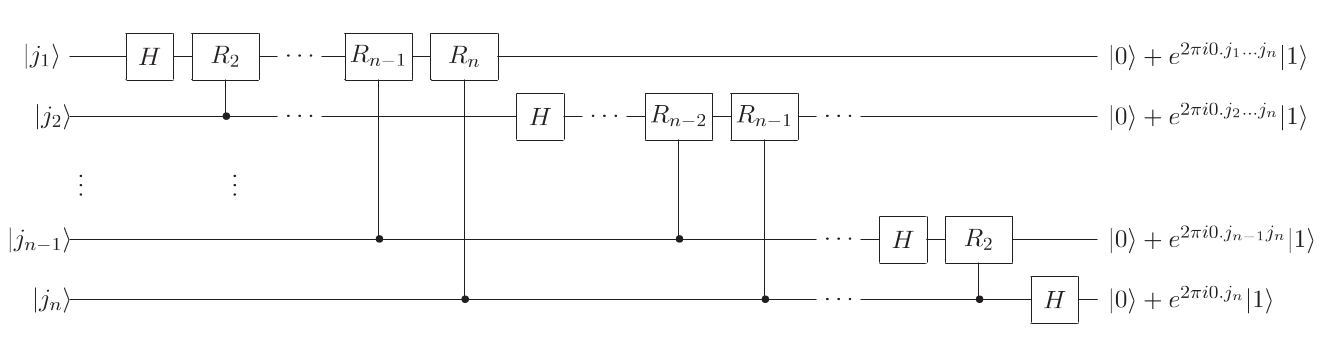
\includegraphics[width=\linewidth]{images/quantumFourierCircuit.png}
    \caption{Here $R_k=\begin{bmatrix}
        1 & 0 \\ 0 & e^{2\pi i/2^k}
    \end{bmatrix}$}
    . This circuit efficiently computes quantum fourier transform.
    \label{fig:quantumFourierCircuit}
\end{figure}
In this, a total of $n(n-1)/2$ gates are required, and atmost $n/2$ swaps are required at the end. Thus providing a $\Theta(n^2)$ algorithm. Unfortunately,  amplitudes in a quantum computer cannot be directly accessed by measurement. Thus, there's no way of determining Fourier transformed amplitudes of the original state.

\section{Phase estimation}
